\documentclass[a4paper, titlepage]{report}

\usepackage[T1]{fontenc}
\usepackage[spanish,activeacute]{babel}
\usepackage[dvipsnames]{xcolor}
\usepackage{lmodern}
\usepackage{graphicx}
\usepackage{caption,subcaption}
\usepackage{hyperref, url}
\usepackage{minted}
\usepackage{listings}
\usepackage{tcolorbox}
\tcbuselibrary{minted}
\usepackage{multicol}
\usepackage{tikz}
\usetikzlibrary{patterns,decorations.pathreplacing}
\usepackage{tabularx}
\usepackage{amsmath}
\usepackage{fmtcount}
\usepackage{booktabs}

\usepackage[left=3cm,right=3cm,top=3cm,bottom=3cm]{geometry}

\definecolor{brown-asm}{HTML}{870000}

\title{
	\textsc{\Large{}\raggedleft{Instalación y Reemplazo de Componentes Internos}}\\
		 \vspace{18pt}
		\fontsize{40}{40}{\textbf{\texttt{LC-3}}}\\
		\Huge\textbf{\textit{Un lenguaje de bajo nivel}}
\vspace{-10pt}
}
\author{\Large{}Ariel Leonardo Fideleff}
\date{junio de 2022}

\begin{document}
	\pagenumbering{gobble}
	\maketitle
	
	\pagenumbering{arabic}
	\thispagestyle{plain}
	\tableofcontents
	
	\chapter{Introducción}
	
	\section{¡Bienvenido al bajo nivel!}
	
	\textit{¡Bienvenido al bajo nivel!}... pero paremos un segundo, ¿qué es el \textit{bajo nivel}? ¿De qué estamos hablando? Si hay un bajo nivel, también debe haber un \textit{alto nivel}, no? ¿Cómo tiene que ver todo esto con la programación?
	
	La verdad es que si bien podríamos estar ya mismo empezando a explicar un programa de ejemplo en \texttt{LC-3}, hay varios conceptos que probablemente tengamos que aclarar sobre el funcionamiento de las computadoras y algo de terminología.
	
	Ya sabemos... probablemente piensan que es aburrido. Pero creemos que si entienden algunos de estos conceptos, puedan también comprender el motivo de las limitaciones y desafíos que conlleva programar con lenguajes de bajo nivel, y del proceso lógico que lleva hacer programas en, concretamente, \texttt{LC-3}. 
	
	\section{Desde el \textit{hardware}}
	
	¿Alguna vez se preguntaron cómo un procesador formado por millones diminutos transistores de silicio es capaz de correr el juego que tanto les gusta? Si alguno se quedó en la parte de \textit{millones de transistores}, simplemente vean la imagen en la figura \ref{fig:die-img} que muestra la estructura interna de un procesador moderno.
	
	\begin{figure}[h]
		\centering
		\captionsetup{justification=centering}
		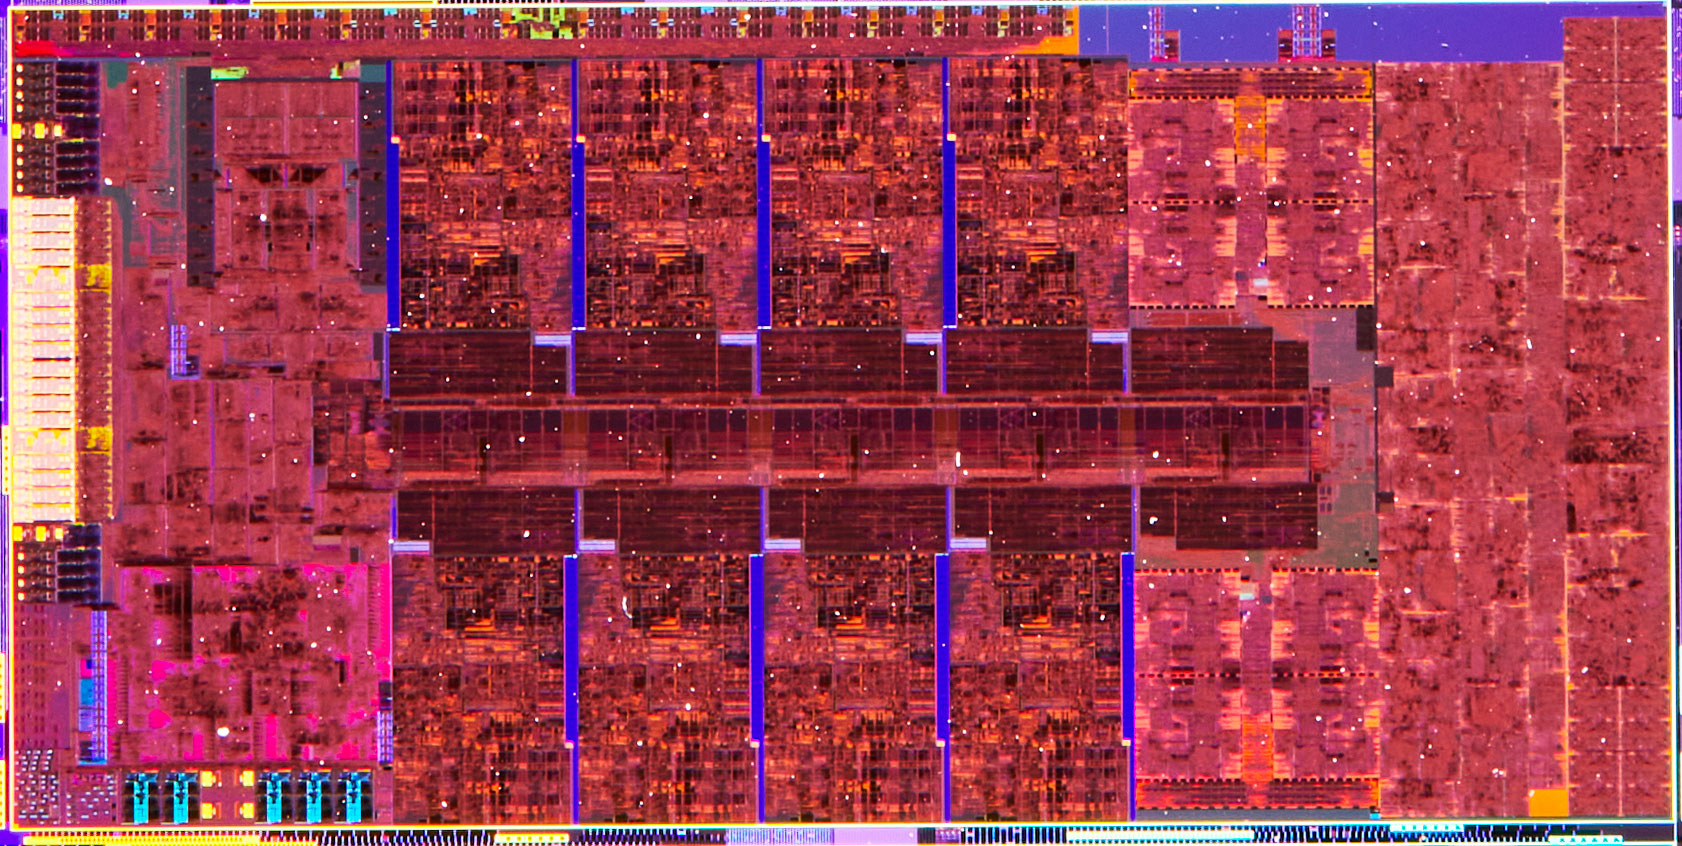
\includegraphics[width=.6\linewidth]{i9-die.jpg}
		\caption{Los millones de transistores que componen un procesador moderno, en este caso el Intel Core i9-12900K}
		\label{fig:die-img}
	\end{figure}

	No se fijen tanto en los colores, su propósito es fundamentalmente distinguir la densidad de transistores en un área determinada.
	
	A lo que apuntamos es que se empiecen a preguntar sobre todo el proceso que conlleva partir desde pulsos eléctricos, a los usos que le damos en el día a día a las computadoras (ya sea en el formato de torre de escritorio, una notebook, o un celular).
	
	Con esto en cuenta, es desde esa placa de silicio que parte todo. Todos los programas que forman el \textit{software} deben de correr en un \textit{hardware} que sea capaz de soportarlos. Y un procesador es \textit{literalmente} una parte central en un sistema de computadora\footnote{Lo entienden? CPU? \textbf{Central} Processing Unit? sigh...}.
	
	Nuestra tarea como programadores de bajo nivel es tener algunas nociones sobre el funcionamiento del hardware, con el fin de luego hacer uso de ese conocimiento, para poder confeccionar software que sea capaz de transmitirle correctamente las instrucciones necesarias para ejecutar las tareas que queramos realizar. 
	
	\section{El \texttt{ISA} y elementos de una computadora}
	
	Ya se van a dar cuenta que una de las cosas que más les gusta a los informáticos es ponerle abreviaturas a todas las cosas, más aún si nos referimos a cosas complejas con nombres largos y difíciles de recordar. Sin embargo, siempre traten de entender al menos qué es de lo que están hablando, antes que usar las abreviaturas por el resto de su vida.
	
	\subsection{El set de instrucciones}
	
	Cuando hablamos de procesadores, si bien, por ejemplo, te pueden vender la cantidad de núcleos que tienen, a nosotros nos interesa más saber que un procesador maneja tareas tales como el manejo de operaciones lógicas y matemáticas, como también el manejo de la entrada y la salida de información (conocida típicamente como \texttt{I/O}, de \textit{Input/Output} en inglés).
	
	Estas tareas son posibles a partir del \textbf{set de instrucciones} que el procesador es capaz de entender y llevar a cabo. \\
	
	Una de las cosas más difíciles al enseñar programación, es transmitir cómo uno debe desglosar en pequeñas subtareas, aquello que alguien normalmente hace intuitivamente en una hoja de papel. Por ejemplo, si nos dicen de hacer un programa en \texttt{C} para contar la cantidad de números impares en un arreglo de números, hay que pensar en cada uno de los pasos que hacemos si nos dieran el mismo problema para hacer con papel y lápiz. Así nos daremos cuenta que en nuestra cabeza, rápidamente \textit{iteramos} por cada uno de los números de la lista mientras los leemos, verificando en cada caso la condición pedida, y luego transmitimos un resultado, ya sea de forma escrita o hablada.
	
	Por lo tanto, a la hora de diseñar un procesador, el objetivo es incluir un conjunto de tareas o \textit{instrucciones} elementales, que combinadas brinden la flexibilidad necesaria para realizar cualquier tarea que queramos que una computadora lleve a cabo.
	
	Así, el \textit{set de instrucciones} de un procesador abarca las distintas instrucciones que es capaz de comprender, y que están resueltas a nivel del hardware. Estas operaciones, como dijimos, se relacionan con operaciones matemáticas (suma, multiplicación), como también con I/O (lectura y escritura en memoria, acceso a registros).
	
	\subsection{¿Y la definición?}
	
	De todas formas, probablemente habrán notado que todavía no definimos el significado de \texttt{ISA}, y eso que habíamos dicho que no había que abusar de las abreviaturas.
	
	El \textbf{Instruction Set Architecture} define un modelo abstracto fundamental de una computadora, y nos da la información de los elementos que tenemos a disposición como programadores para que nuestro software pueda interactuar con los componentes (a lo que haría al hardware) definidos por la arquitectura. Para que quede claro, la \textbf{arquitectura de una computadora} es, a modo general, el diseño de cómo va a funcionar: la interacción entre sus distintos componentes, las reglas que lo rigen y algunos detalles sobre su posible implementación (es decir, cómo lo llevamos a cabo en un escenario real). La forma concreta en que se implementa un ISA para un procesador dado se lo conoce como \textbf{microarquitectura}.
	
	Así podemos decir que el \textit{ISA} y la \textit{microarquitectura} son áreas dentro de lo que abarca la \textit{arquitectura de una computadora}.
	
	En términos simples, el ISA especifica la parte de la arquitectura sobre qué es lo que se encuentra a disposición del programador para poder decirle a la computadora qué es lo que tiene que hacer. Es por esto que antes habíamos introducido el concepto del set de instrucciones, ya que es una de las partes principales del ISA. Reiteramos, es \textit{una de las partes principales}, pero esto no implica que sea todo.\\
	
	\subsection{¿Cómo nos llega la información?}
	\label{sec:isa-io}
	
	Ya veremos que una de las instrucciones de \texttt{LC-3} es \texttt{ADD}, el cual uno puede asumir que sirve para sumar dos números. Ahora bien, pensá que un amigo te dice literalmente ``\textit{sumá dos números}''. Lo primero que uno responde es, ``\textit{¿qué números?}''. Entonces te apunta a una hoja de papel, desde la cual tenés que leer los números.
	
	Observar que tenemos que saber cómo manejar una hoja de papel para poder leer la información en ella. Podrá parecer trivial, pero es que intuitivamente sabemos cómo agarrar una hoja de papel, y disponerla frente a nuestros ojos para leer lo que esté allí escrito. Y una vez la tenemos frente a nuestros ojos, sabemos cómo interpretar lo que vemos de una forma que nuestro cerebro lo pueda comprender.
	
	Esto ilustra que las operaciones de por sí no son suficientes para que una computadora sepa lo que tiene qué hacer. De hecho, básicamente estaríamos ignorando completamente la definición de ``informática'', que entre tantas cosas abarca al \textit{conjunto de técnicas para el procesamiento, almacenamiento y transmisión de la información}. Necesitamos que la computadora sepa \textit{cómo leer} la información, así también \textit{cómo devolverla}. Por lo tanto, el ISA especifica también la forma en la que se ingresa y se presenta la información procesada al sistema, el I/O ya mencionado.
	
	La respuesta simple a la pregunta en el caso de una computadora es bueno, a través de \textit{pulsos eléctricos}. Pero... ¿cómo se ingresan esos pulsos eléctricos? ¿cómo se interpretan? ¿definen algún patrón? Las preguntas concretas sobre cómo implementarlo se las dejamos a los encargados de diseñar la arquitectura y el hardware, pero como programadores nos interesa la especificación de instrucciones que nos permitan leer y mostrar información, es decir, saber cómo usar las instrucciones que nos habilitan el I/O.
	
	En el caso de nuestro ejemplo, tenemos que tener las ``instrucciones'' para que nos digan cuando se quiere, por ejemplo, leer de un papel, y que sepamos hacerlo.
	
	\subsection{¿Cómo guardamos la información?}
	\label{sec:isa-memory-intro}
	
	Una vez que pudimos leer la información, debemos de tenerla guardada en algún lugar para poder operar con ella. Esto introduce otro componente importante de una computadora, la \textbf{memoria}.
	
	En nuestro ejemplo nos dan una hoja de papel donde podemos decir que ``están almacenados'' los números, así que lo podemos considerar como un ejemplo de memoria, no? No hay que confundir la memoria con \textit{medios de almacenamiento}. De ahora en más, cuando hablemos de memoria, siempre haremos referencia a sistemas o dispositivos que nos permitan almacenar información \textbf{para su uso inmediato}.
	
	Mírenlo de esta forma: es más rápido sumar dos números cuando los tenemos ya en nuestra cabeza, que si estamos constantemente leyéndolos del papel. La memoria en este caso es nuestra capacidad de recordar los números con los que operamos, y el papel es un medio de almacenamiento que nos permite resguardar los números a largo plazo. Análogamente, esto se relaciona en cómo es más rápido leer de la memoria RAM, que de un medio de almacenamiento como un disco duro HDD o hasta un disco de estado sólido SSD.\\
	
	Dicho esto, para operar con los números, es necesario tener alguna forma de que los números permanezcan en nuestra cabeza, al menos de forma temporal. Si queremos hacer $2+2$, tenemos que acordarnos, por más que sea por fracciones de segundo, de los dos números, para saber e informar que el resultado de la operación es $4$. Así, es que el ISA define también cómo podemos acceder a la memoria, cómo podemos operar con ella, y las instrucciones relacionadas.\\
	
	En las computadoras hay distintos tipos de memoria que ocupan distintos lugares en una jerarquía que depende según su velocidad, aunque trataremos estas diferencias más adelante cuando definamos en detalle el ISA de \texttt{LC-3}.
	
	Nomás tengan en cuenta que cuando hablamos de ``memoria'' muchas veces no sólo nos referimos, como ya habíamos aclarado, a memorias de uso inmediato, sino concretamente a memorias volátiles (que no permiten almacenar información a largo plazo y que se borran cuando, por ejemplo, se les quita energía) a las cuales podemos acceder a sus contenidos de forma aleatoria (modificar y acceder a distintas partes de la memoria rápidamente). Hoy en día, este tipo de memorias las conocemos como \textit{memorias RAM} (Random Access Memory, en español, memorias de acceso aleatorio).
	
	Créannos que a lo largo de este texto se les va a ir aclarando de lo que estamos hablando.
	
	\subsection{¿La operación se guarda?}
	\label{sec:isa-memory}
	
	Entonces ya sabemos leer los números, guardarlos, hacer la operación, y devolver el resultado. ¿Nos falta algún paso más?
	
	En vez de dar una respuesta, vamos a proponer otra pregunta: ¿La operación dónde está guardada? Dicho de otra forma, ¿de dónde lee la computadora la operación?
	
	La respuesta lógica a esta pregunta es que la operación se encuentra en un programa, y ese programa necesariamente tiene que estar en la memoria. Al fin y al cabo, el programa es con el cual estamos haciendo operaciones en el uso inmediato.
	
	Pero en la memoria también habíamos guardado los números una vez los habíamos leído. Esto nos lleva a la pregunta: ¿cómo distinguimos la memoria en dónde está nuestro programa, con la memoria de la información que leímos?
	
	Tantas preguntas y pocas respuestas...\\
	
	Cuando queremos acordarnos de alguna cosa, generalmente sólo ``lo pensamos'' y con suerte nos acordamos y podemos utilizar la información obtenida. Si bien los científicos podrán no saber con exactitud todavía cómo funciona este proceso, mientras tanto tenemos que tener alguna forma de diseñar una memoria que nos permita acceder a los distintos fragmentos de información que contiene de una forma ordenada. Es por esto que la memoria tiene \textbf{direcciones de memoria}, que funcionan como identificadores para cada uno de los sectores de la memoria que podemos acceder de forma independiente según nuestras necesidades. 
	
	Notar que cada dirección de memoria se corresponde con una cantidad fija de espacio. Es decir, es como si dividiéramos la memoria en millones de pedazos iguales, y que cada uno de ellos sea accesible por una dirección de memoria. Típicamente en las computadoras de hoy en día, cada uno de estos pedazos tiene el tamaño de 1 \textit{byte}, el equivalente a 8 \textit{bits}. De todas formas, veremos que en el caso de \texttt{LC-3}, la memoria es ``16-bit addressable'', es decir, que cada pedazo tiene 16 bits.
		
	Para el que se encuentre perdido en este sentido, probablemente hayan visto que los archivos en la computadora tienen un determinado tamaño. Un documento de texto tiene un tamaño en el orden de los \textit{kilobytes}, una imagen en el orden de los \textit{megabytes}, y una película probablemente en el orden de los \textit{gigabytes}. Son todas unidades de escala basadas en los bytes. Y para que sepan, cada bit es literalmente un 0 o un 1, por lo que si hablamos de 12 kilobytes (kB), es lo mismo que decir $12 * 1000 = 12\,000$ bytes, también equivalente a $12.000 * 8 = 96\,000$ bits, o sea, un conjunto de $96\,000$ 0s y 1s. No confundir los kilobytes con los $kibibytes$, esos se multiplican por $1024$ cada paso, en vez de por $1000$.\\
	
	Igual nos estamos yendo del tema. A lo que vamos es que la memoria está dividida en pedazos para que podamos accederla y modificarla fácilmente. Si bien hablamos de archivos para ilustrar la idea de los tamaños, estos ocupan espacio en un medio de almacenamiento, el cual ya habíamos diferenciado de la memoria. Comúnmente los programas se encuentran almacenados  en medios de almacenamiento no volátiles (justamente, por ejemplo, un disco duro), y a la hora de ejecutarlos se cargan en memoria, que es de uso inmediato.
	
	Al cargarse el programa en memoria podemos saber las direcciones que ocupa, como también las direcciones en las cuales se leyó la información a procesar, en este caso, los números a sumar. Así, una de las piezas que nos falta para resolver nuestro problema, es cómo indicarle al programa en qué parte de la memoria se encuentran los números ingresados. Estas distintas formas de indicar direcciones de memoria en el programa, se las llama \textbf{addressing modes} (en español, \textit{modos de direccionamiento}, y también se encuentran especificados en el ISA.
	
	De forma simplificada, podríamos decir que la información se encuentra a una cierta cantidad de direcciones de memoria de distancia desde la ubicación de la instrucción en memoria, como también podríamos especificar concretamente la dirección de memoria de forma absoluta. Todo dependerá del contexto con el que estemos trabajando en nuestro programa. Más adelante veremos los addressing modes de los cuales disponemos con \texttt{LC-3}.
	
	\subsection{¿De qué forma tengo que entender esos 1s y 0s?}
	
	Ya sabemos que se está haciendo largo. No se preocupen, ya casi estamos terminando. Al menos les sirve para entender lo compleja que es una computadora, sin mencionar que estamos simplificando el proceso para que sea más ameno y fácil de entender.\\
	
	Una vez que el programa sabe en qué lugar de la memoria encontrar los números con los cuales operar, afortunadamente y como ya mencionamos, es común que exista una instrucción para poder sumar dos números. Sin embargo, ¿cómo sabe el programa cómo interpretar esos números?
	
	Otra cosa que nos parece intuitiva es que el símbolo \textit{6} represente el número dicho. Aunque también sabemos que \textit{seis} representa lo mismo. Y en números romanos, sucede con \textit{VI} de igual forma.
	
	De la misma forma que tenemos varias maneras de hablar de lo mismo, también es así con las computadoras. Nuevamente, los \textbf{data types} (\textit{tipos de datos}, en español) están también definidos en el ISA, y haremos uso de ellos según nos sea más conveniente. Un tipo de dato común en programación es la representación de los números en \textit{binario}, lo cual naturalmente se da por lo que ya venimos explicando, que los procesadores están compuestos de transistores, y que su estado de encendido o apagado representa un 1 o un 0 respectivamente. También la representación de la información como conjuntos de bits en la memoria, y en general el uso de lógica binaria a lo largo de un sistema de computadora facilita las distintas tareas como programadores.\\
	
	Para el caso de \texttt{LC-3}, veremos que sólo tenemos a disposición una única forma de representar los datos: como enteros en \textbf{complemento a 2}. Debido a que por ahora no entraremos en los detalles, podemos asumir para nuestro problema que la instrucción de suma que usaremos, ya sabe cómo están representados los números a sumar en la memoria.
	
	\subsection{Pasando en limpio}
	
	Tras explicar todas las distintas partes (a modo general) que forman parte del proceso para que una computadora pueda hacer una tarea que nos puede parecer tan básica como sumar dos números, intentaremos resumir lo que aprendimos, para continuar con las ideas claras.\\
	
	En resumen:
	
	\begin{itemize}
		\item La operación de suma se encuentra como una instrucción en un programa el cual se carga en la memoria, ubicándose en un conjunto de direcciones de memoria.
		\item El programa debe de contener, y hacer uso, de las instrucciones necesarias para leer los números, y almacenarlos en otras posiciones en la memoria.
		\item Al guardarse los números, éstos quedan representados con un determinado tipo de dato, el cual el programa tiene que tener en cuenta a la hora de hacer la operación.
		\item Así, a la instrucción de suma se le indican dónde se encuentran los números guardados mediante un modo de direccionamiento, el cual apunta a las direcciones correspondientes de memoria. La operación es capaz de entender la forma en la cual aquellos números se encuentran allí representados.
		\item Tras ejecutar la instrucción de suma, el resultado debe ser almacenado en otro lugar de la memoria.
		\item Finalmente, debe de indicarse la ubicación del resultado antes obtenido, para que éste sea informado al usuario mediante un dispositivo de salida adecuado, con las instrucciones correspondientes para este propósito.
	\end{itemize}

	Así parece más sencillo, ¿no? Con esta idea aproximada del proceso, esperamos que puedan seguirnos mejor mientras exploramos las particularidades de \texttt{LC-3}, su ISA y los programas que estaremos desarollando para este \textit{lenguaje de bajo nivel}.

	\section{Una vez más, ¿qué significa \textit{alto} y \textit{bajo} nivel?}
	
	Volvemos a la pregunta del comienzo del capítulo, para resolver de una vez la incógnita: \textbf{¿qué es un \textit{lenguaje} de bajo nivel?}
	
	Para que se sientan más familiares con lo que vamos a hablando, vamos a estar comparando o relacionando lo que expliquemos con el lenguaje \texttt{C}, el cual ya probablemente conocen por su trayecto en la escuela. Al fin y al cabo, es más sencillo partir desde lo que ya saben, que explicar todo desde cero.\\
	
	Capaz una forma distinta de pensarlo, sin dar muchas vueltas más es:
	
	\begin{center}
		\textit{¿por qué necesitamos ahora saber todo esto de sobre cómo funciona una computadora, y lo ignorábamos cuando programábamos en \texttt{C}?}
	\end{center}
	
	Primero y principal, capaz sería muy agobiante dar todo esto en 3er año. Además, la idea es dar esto a quienes eligieron la especialidad y a los cuales esta información sea relevante si luego pretenden desempeñarse como Técnicos en Informática Personal y Profesional.
	
	Pero más allá de los detalles del cursado, en la pregunta precisamente radica la diferencia entre un lenguaje de bajo nivel, y uno de alto nivel.
	
	\subsection{\texttt{C} es un lenguaje de alto nivel...}
	
	...casi. Un \textbf{lenguaje de alto nivel} es aquel que provee una abstracción respecto del funcionamiento interno de la computadora. En este sentido, es común que un lenguaje de alto nivel haga uso de vocabulario o elementos del lenguaje hablado, que faciliten expresar los programas que queremos desarrollar.
	
	Esto lo podemos ver a partir de estructuras de control como \texttt{if} (``si'' en inglés) o \texttt{while} (``mientras'', en inglés), entre otras. Cuando usamos estos elementos, no es necesario conocer las instrucciones del procesador, ni el manejo de la memoria, brindándonos mayor flexibilidad y, en cierta forma, haciendo que sea más legible para un principiante o alguien que simplemente no sepa de programación.
	
	Si creen que \texttt{C} no es muy fácil de leer, pueden ver el ejemplo de otros lenguajes de alto nivel como \texttt{COBOL}, diseñado hace más de 60 años con el objetivo de ser lo más parecido posible a la habla inglesa. 
	
	\begin{figure}[h]
		\centering
\begin{tcblisting}{listing engine=minted, minted language=cobolfree, listing only, hbox}
IDENTIFICATION DIVISION.
PROGRAM-ID. HELLOWRD.

PROCEDURE DIVISION.
DISPLAY "HOLA MUNDO".
STOP RUN.
\end{tcblisting}
		\caption{Ejemplo de programa ``Hola Mundo'' hecho en \texttt{COBOL}}
	\end{figure}

	Dicho esto, el motivo por el cual decimos que \texttt{C} es \textit{casi} un lenguaje de alto nivel, es porque el concepto de ``alto nivel'' de cierta forma puede depender del contexto. Por definición, \texttt{C} es un lenguaje de alto nivel, y es totalmente entendible si lo comparamos con \texttt{LC-3}. Sin embargo, si tenemos en cuenta, más allá del ejemplo de \texttt{COBOL}, el caso de lenguajes más nuevos como \texttt{Javascript} o \texttt{Python}, estos últimos brindan un nivel superior de abstracción que \texttt{C}.
	
	Por ejemplo, una de las tareas principales programando en \texttt{C} es el manejo de la memoria. Además, mucho código que interactúa directamente con el hardware de la computadora se escribe en \texttt{C}. Parte del kernel de Linux está escrito en \texttt{C}!\\
	
	De esta forma, como podemos ver, cuando hablamos si que a uno ``le gusta el alto/bajo nivel'' o de la diferencia entre lenguajes de \textit{alto} y \textit{bajo} nivel, es una manera en la que nos referimos a qué tanta abstracción brinda el lenguaje con respecto a los detalles específicos del hardware que utilizamos.
	
	Cerrando el tema con \texttt{C}, al ser de ``alto nivel'' requiere un compilador que traduzca el código escrito, en código de máquina que la computadora pueda interpretar. Es decir, traducir en instrucciones del procesador concreto donde lo compilemos, como también depende del sistema operativo, y de otros elementos que hacen especial a la computadora donde trabajamos. También por esto, por lo general el código de \texttt{C} es ``portable'' entre distintas plataformas, ya que mientras exista un compilador que pueda traducir el código fuente en código de máquina para el caso en el que lo necesitemos, podremos (generalmente) recompilar el programa según se lo necesite.
	
	Cuando instalamos un programa, es común descargar lo que se conocen como los \textit{binarios} o \textit{ejecutables}, es decir, el código ya compilado. Como hoy en día la mayor parte de la interacción con el hardware está resuelta a través del sistema operativo, uno tiende a encontrar que puede descargar versiones para Mac, Windows o Linux. Estas versiones están compiladas por separado ya que requieren de interfaces diferentes para poder intermediar con el sistema operativo en realizar las tareas para las que los programas están destinados.
	
	Además, ayuda en este sentido que hoy en día la mayoría de los procesadores de computadora usan una arquitectura común: \texttt{x86\_64}. Puede que alguna vez hayas visto, aunque haya cobrado menos sentido en los últimos años, que ciertos programas son solo compatibles con procesadores de ``64 bits''.  De ahí viene el ``64'' del nombre, ya que esta arquitectura es una versión ``de 64 bits'' de la arquitectura \texttt{x86}. Para no irnos más de tema, lo dejamos a su voluntad si quieren investigar más al respecto.
	
	
	\subsection{¿Qué es \texttt{LC-3}?}
	
	Creemos que a este punto quedó más que claro que \texttt{LC-3} es un lenguaje de bajo nivel, no? Un segundo... hay una pregunta más importante que todavía nos falta por hacer. \textbf{¿Qué es \texttt{LC-3}?}
	
	¡Las abreviaturas \textit{strike again}! \texttt{\textbf{LC-3}} son las iniciales de \textbf{Little Computer 3}, en español, \textit{Pequeña Computadora 3}. Podrán deducir que con un nombre parecido al de una película, el \textit{3} está ahí porque \texttt{LC-3} es la tercera iteración de algo. En este caso, la tercera versión de una \textbf{arquitectura}, que utilizamos con fines educativos para empezar a aprender a programar en \texttt{Assembly}.\\
	
	Pero entonces... si \texttt{LC-3} es una arquitectura, \textit{¿cómo es también un lenguaje?}
	
	Cuando diseñamos una arquitectura, ésta define un conjunto de instrucciones y herramientas disponibles al programador, que nos permiten poder correr programas en un procesador que implemente el ISA. Dichas herramientas determinan, al fin y al cabo, un lenguaje con el que tenemos que hablar con la computadora para que ésta pueda entender lo que le estamos diciendo.
	
	¿Recuerdan cuando en la sección \ref{sec:isa-io} nos preguntábamos si los pulsos electricos que nos llegaban en la entrada formaban algún patrón? Bueno, pensemos esto para el caso de las instrucciones que le llegan al procesador. De alguna forma, los pulsos eléctricos que le transmitimos, los 0s y 1s que viajan, deben indicarle al procesador que ejecute la instrucción \texttt{ADD}, por ejemplo. Aquellos detalles, están definidos en el ISA. Y el patrón de aquellos bits, que utiliza nuestro programa como directivas al procesador, son en cierta forma, un \textit{lenguaje}, una forma de comunicarnos con la computadora.\\
	
	\subsection{\texttt{LC-3}, un lenguaje de bajo nivel}
	\label{sec:lc3-low-level}
	
	Habiendo entendido un poco mejor \textit{qué} es \texttt{LC-3}, ahora vamos a cerrar con el concepto de lenguaje de \textit{bajo nivel}.
	
	Mientras que un lenguaje de \textit{alto nivel} nos abstrae de los detalles sobre el funcionamiento interno de la computadora, un \textbf{lenguaje de bajo nivel}, en su contraparte, prácticamente no provee abstracción alguna del ISA, a lo que se encuentra íntimamente relacionado con las instrucciones y la estructura que el ISA define. Por este motivo, más allá de que pueda llamársele a lenguajes como \texttt{C} ser de bajo nivel en comparación con otros, en general al hablar del bajo nivel nos referimos al \textbf{código de máquina}, o el \textbf{código \texttt{Assembly}}.
	
	Para aquel que no haya visto nunca un fragmento de código de bajo nivel, vamos a adelantarnos un poco y tomar el ejemplo de la instrucción \texttt{ADD}. Como recordarán de la sección \ref{sec:isa-io}, la instrucción \texttt{ADD} permite sumar dos números en el lenguaje de \texttt{LC-3}. El nombre de la instrucción está así definido en su ISA, y es aquel con el cual la invocamos en código \texttt{Assembly}.
	
	\begin{figure}[h]
		\centering
\begin{tcblisting}{listing engine=minted, minted language=gas, listing only, hbox}
ADD	R0, R1, R2
\end{tcblisting}
	\caption{Ejemplo de instrucción de suma en \texttt{Assembly} de \texttt{LC-3}}
	\label{fig:add-asm-example}
	\end{figure}

	La Figura \ref{fig:add-asm-example} nos muestra un ejemplo de cómo usaríamos la instrucción \texttt{ADD}, dentro del código de \texttt{Assembly} de \texttt{LC-3}. En aquel caso, se está indicando que se sumen los números contenidos en los \textit{registros} \texttt{R1} y \texttt{R2}, y que el resultado de la operación se guarde en el registro \texttt{R0}. Más adelante explicaremos qué son, y el rol que cumplen los registros. Por el momento queremos que vean y vayan pensando, cómo todos los conceptos que venimos aprendiendo se plasman el código de un programa.
	
	Además, también podríamos representar la misma instrucción con su código de máquina correspondiente, tal como se muestra en la Figura \ref{fig:add-machine-example}.
	
	\begin{figure}[h]
		\centering
		\begin{tikzpicture}[scale=.75]
				\draw (0,0) -- (16,0) -- (16,1.5) -- (0,1.5) -- cycle;
				\draw (0,1.5) -- (0,1.75); 
				\draw (4,0) -- (4,1.75);
				\draw (7,0) -- (7,1.75); 
				\draw (10,0) -- (10,1.75);
				\draw (11,0) -- (11,1.75);
				\draw (13,0) -- (13,1.75);
				\draw (16,0) -- (16,1.75);
				\path (0,1.5) -- node [yshift=-4pt,label={15}]{}(1,1.5);
				\path (3,1.5) -- node [yshift=-4pt,label={12}]{}(4,1.5);
				\path (4,1.5) -- node [yshift=-4pt,label={11}]{}(5,1.5);
				\path (6,1.5) -- node [yshift=-4pt,label={9}]{}(7,1.5);
				\path (7,1.5) -- node [yshift=-4pt,label={8}]{}(8,1.5);
				\path (9,1.5) -- node [yshift=-4pt,label={6}]{}(10,1.5);
				\path (10,1.5) -- node [yshift=-4pt,label={5}]{}(11,1.5);
				\path (11,1.5) -- node [yshift=-4pt,label={4}]{}(12,1.5);
				\path (12,1.5) -- node [yshift=-4pt,label={3}]{}(13,1.5);
				\path (13,1.5) -- node [yshift=-4pt,label={2}]{}(14,1.5);
				\path (15,1.5) -- node [yshift=-4pt,label={0}]{}(16,1.5);
				\foreach \x in {0,...,16}
					{\draw (\x,1.5) -- (\x,1.25); \draw (\x,0) -- (\x,0.25);}
					
				\def\array{0,0,0,1,  0,0,0,   0,0,1,   0,0,0,    0,1,0}
				\foreach [count=\i] \x in \array
					{\path (\i-1,.75) -- node [midway] {\Large \x} (\i,.75);}
					
				\draw [thick,decoration={brace,mirror,raise=4pt},decorate] (0.05,0) -- (3.95,0) node[midway,below,yshift=-8pt] {\texttt{\textcolor{blue}{ADD}}}; 
				\draw [thick,decoration={brace,mirror,raise=4pt},decorate] (4.05,0) -- (6.95,0) node[midway,below,yshift=-8pt] {\texttt{\textcolor{brown-asm}{R0}}}; 
				\draw [thick,decoration={brace,mirror,raise=4pt},decorate] (7.05,0) -- (9.95,0) node[midway,below,yshift=-8pt] {\texttt{\textcolor{brown-asm}{R1}}}; 
				\draw [thick,decoration={brace,mirror,raise=4pt},decorate] (13.05,0) -- (15.95,0) node[midway,below,yshift=-8pt] {\texttt{\textcolor{brown-asm}{R2}}}; 
		\end{tikzpicture}
		\caption{Ejemplo de instrucción de suma en \textit{código de máquina} de \texttt{LC-3}}
		\label{fig:add-machine-example}
	\end{figure}
	
	En la figura en cuestión ya podrán observar algunas cosas más de las que hablamos, como que la longitud de la instrucción completa ocupa un total de 16 bits, lo que haría que abarque el tamaño de una dirección de memoria (recordemos que en \texttt{LC-3} la memoria es ``16-bit addressable'', [Sección \ref{sec:isa-memory}]). Además, podemos ver que los registros antes nombrados en \texttt{Assembly} (\textcolor{brown-asm}{\texttt{R0}}, \textcolor{brown-asm}{\texttt{R1}} y \textcolor{brown-asm}{\texttt{R2}}), para el código de máquina los representamos en binario.
	
	Para no dejar dudas (el subíndice representa la base en la que se encuentra el número): \vspace{3pt}
	
	\noindent\begin{tabularx}{\textwidth}{>{\centering\arraybackslash}X >{\centering\arraybackslash}X >{\centering\arraybackslash}X}
		$000_2 = 0_{10}$ & $001_2 = 1_{10}$ & $010_2 = 2_{10}$
	\end{tabularx}\\
	
	En el próximo capitulo estaremos desarollando el detalle de cada una de las instrucciones de \texttt{LC-3}.
	
	Más allá de esto, como pueden ver, tanto con código de máquina como con \texttt{Assembly}, en ambos casos hacemos uso de operaciones relacionadas con el ISA, casi sin abstracciones respecto a la arquitectura. Como mucho y como también veremos, \texttt{Assembly} le da mayor legibilidad al código respecto al código de máquina (binario), entre otros elementos útiles por conocer.
	
	\section{Felicitaciones! Lo que nos espera el próximo capítulo}

	Enhorabuena, con toda esta introducción teórica, ya deberían tener todo lo necesario para adentrarnos en mayor profundidad, en los detalles del ISA de \texttt{LC-3}.
	
	% TODO: Revisar que esté bien esto
	Nos veremos en el próximo capítulo con todo lo que necesitan saber sobre las instrucciones que tienen a su disposición, el funcionamiento de la memoria, detalles sobre los registros, I/O, llamadas al sistema, el stack, y ejemplos de cómo implementar desde estructuras básicas en programación (que ya probablemente hayan visto en \texttt{C}) como operaciones aritméticas, loops e ifs, hasta casos de uso más avanzados como subrutinas y recursión.
	
	% TODO: Assembler vs Assembly
	
	% TODO: Al explicar Assembly, destacar el buen uso de los .FILL al ejecutar el programa -> mostrar como un .FILL puede dar OVERFLOW y romper programa (caso Fibonacci grande?)
	% TODO: Hacer programa Fibonacci pero con I/O!!!!
	
	% TODO: Nombrar emulador web https://wchargin.com/lc3web/
	\chapter{El \texttt{ISA} de \texttt{LC-3}}
	
	Recordando un poco lo visto en el capítulo anterior, el \textit{Instruction Set Architecture} define los elementos que tenemos a disposición como programadores para que podamos escribir código que le permita a la computadora ejecutar las tareas que queramos. Con esto en cuenta, vamos a desarrollar qué es lo que nos ofrece el ISA de \texttt{LC-3}, y cómo podemos utilizarlo para desarrollar programas.
	
	Les aseguramos que lograr sumar dos números en un lenguaje de bajo nivel es mucho más emocionante que lograr lo mismo en \texttt{C}.
	
	Recomendamos hacer uso del simulador online de \texttt{LC-3} para experimentar con los conceptos que iremos desarrollando en el capítulo: \url{https://wchargin.com/lc3web/}. Más información sobre su uso en el Capítulo 3.
	
	% TODO: Usar .BLKW?
	\section{El acceso a la memoria}
	
	Para poder empezar a programar en el lenguaje de \texttt{LC-3}, debemos entender mejor el funcionamiento de una de las partes clave su ISA: la \textbf{memoria}. O más bien, vamos a estar hablando de los distintos elementos de los cuales disponemos para almacenar información.
	
	Generalmente, tendemos a generalizar, y le llamamos ``memoria'' a todo aquel dispositivo o medio que guarda algún tipo de dato. Como ya mencionamos en la Sección \ref{sec:isa-memory-intro}, distinguimos la memoria de los \textit{medios de almacenamiento}, los cuales típicamente no son volátiles. Para continuar con este desglose de qué es concretamente lo que podemos llamar como memoria, lo vamos a diferenciar de los \textit{registros}, los cuales vamos a describir en la Sección \ref{sec:registers}.
	
	\subsection{La memoria}
	
	Como ya venimos adelantando, la memoria, por un lado, es el lugar donde nuestro programa va a estar cargado, y de la cual se van a leer las instrucciones que el procesador va a ejecutar. Por otro lado, también cumple el rol de almacenar la información que se necesita procesar, al igual que posiblemente los resultados generados como producto de las operaciones realizadas.
	
	\subsubsection{Tamaño de una dirección de memoria}
	
	En la Sección \ref{sec:isa-memory}, habíamos mencionado la capacidad de poder acceder a todos los elementos contenidos en la memoria mediante una serie de \textit{direcciones}, que la dividen en muchos pedazos de igual tamaño. Aquellos pedazos, en el caso de \texttt{LC-3}, pueden almacenar hasta 16 bits cada uno, y es por eso que insistimos en llamar a esta memoria ``16-bit addressable''. Otro nombre que también puede recibir en este caso particular es el de ``\textit{word-addressable}'', ya que el \textit{tamaño de palabra} (\textit{word}, en inglés) en \texttt{LC-3} es también de 16 bits. Esta nomenclatura existe para diferenciarse de las memorias más comunes que almacenan hasta 8 bits por dirección, el equivalente a 1 byte, así recibiendo el nombre de ``\textit{byte-addressable}''.
	
	Cabe aclarar que el tamaño o \textbf{longitud de palabra} es, de forma simplificada, la cantidad de bits que el procesador es capaz de procesar en un ciclo de procesamiento\footnote{Concretamente, la cantidad de bits en un ciclo que es capaz de procesar la \textbf{ALU}, \textit{Unidad Artimético-Lógica}, que se encuentra en el procesador y es responsable de llevar a cabo las instrucciones relacionadas con operaciones aritméticas y/o lógicas (como dice su nombre).}. Cada ciclo está definido por la \textit{velocidad de reloj} del procesador en concreto, es decir, la cantidad de operaciones que es capaz de realizar en una unidad de tiempo. Generalmente nos venden esta característica como la ``cantidad de GHz'' a la que operan los núcleos del procesador. Notar que leemos GHz como \textit{gigahertz}, dándose que 1 GHz = $1\,000\,000\,000$ Hz, es decir, $10^9$ operaciones por segundo.
	
	\subsubsection{Direcciones de memoria disponibles}
	
	De todas formas, otro de los parámetros que nos interesa de la memoria no es sólo ``cuánto puede almacenar cada espacio de memoria'' sino la \textit{cantidad} de aquellos espacios.
	
	En el caso de \texttt{LC-3}, en principio, tenemos el acceso a un total de $65\,536$ ($2^{16}$) direcciones de memoria. Esto se da porque, generalmente, si la cantidad de bits necesarios para representar una dirección es menor o igual a la longitud de palabra, éstos pueden ser procesados con mayor eficiencia por el procesador. Véase que al tener $2^{16}$ direcciones, podemos asignarle a cada una, una combinación única de 16 bits.
	
	\begin{figure}[h]
		\centering
		\begin{tikzpicture}[scale=1.25, every node/.style={transform shape}]
			\node[label={[yshift=-12pt, xshift=-1pt]90:\textvisiblespace}] (st) at (0,0) {};
			\foreach [count=\i, evaluate=\x as \y using int(\x/2)]  \x in {0,2}
				{\node[label={[xshift=-0.5pt, gray]0:\fontsize{4pt}{3pt}\selectfont{}\raisebox{.2pt}{$\times$}$2$}]  (c1\i) at (1,-1+\x) {\y}; \draw[-stealth] (st) -- (c1\i);}
			\foreach [count=\i, evaluate=\i as \j using int((\i+1)/2)]  \x in {0,...,3} {
				\pgfmathsetmacro\y{Mod(\x,2)}
				\pgfmathsetmacro\z{Mod(int(\x / 2),2)}
				\node(c2\i) at (2,-1.5+\x) {\pgfmathprintnumber{\z}\pgfmathprintnumber{\y}};
					\draw[-stealth] (c1\j) -- (c2\i);
				}
			\foreach [count=\i, evaluate=\i as \j using int((\i+1)/2), evaluate=\x as \xx using \x/2)]  \x in {0,...,7} {
				\pgfmathsetmacro\p{Mod(\x,2)}
				\pgfmathsetmacro\y{Mod(int(\x / 2),2)}
				\pgfmathsetmacro\z{Mod(int(\x / 4),2)}
				\node (c3\i) at (3.25,-1.75+\xx) {\small\pgfmathprintnumber{\z}\pgfmathprintnumber{\y}\pgfmathprintnumber{\p} $\cdots$ };
				\draw[-stealth] (c2\j) -- (c3\i);
			}
		
			\draw[dashed, gray] (0.8,-2) -- (0.8,2) -- (1.2,2) -- (1.2,-2) -- cycle;
			\node at (1,-2.25) {$2^1$};
			
			\draw[dashed, gray] (1.7,-2) -- (1.7,2) -- (2.3,2) -- (2.3,-2) -- cycle;
			\node at (2,-2.25) {$2^2$};
			
			\draw[dashed, gray] (2.675,-2) -- (2.675,2) -- (3.275,2) -- (3.275,-2) -- cycle;
			\node at (3.,-2.25) {$2^3$};
		\end{tikzpicture}
	 \caption{Visualización de las nuevas combinaciones únicas que se generan al agregar un bit}
\end{figure}

	Es común nombrar las direcciones de memoria con su representación en hexadecimal, ya que es mucho más conciso que usar la representación binaria, e incluso la decimal, de una dirección concreta.	Hay que aclarar que estas son todas formas de representar el mismo número, y no cambian el espacio de memoria al que nos referimos. Al fin y al cabo, siempre habrán $2^{16}$ posibles direcciones, pero en vez de decir que accedemos a la dirección \texttt{\color{Brown}b11000000000000} o la dirección \texttt{\color{Brown}\#12288}, la mencionamos como \texttt{\color{Brown}x3000}. 
	
	Por si se encuentran confundidos al respecto, la representación de un número en \textbf{hexadecimal} hace uso de 16 símbolos, en vez de los 10 a los que estamos acostumbrados en el sistema decimal. Si normalmente representamos los números en ``base 10'', y en binario los representamos en ``base 2'', en hexadecimal usamos ``base 16''.  De esta forma, los primeros 10 símbolos son idénticos al sistema decimal, del \texttt{0-9}. Sin embargo, los 6 restantes abarcan el rango \texttt{A-F}. Así es, usamos letras como parte de este sistema de numeración.
	
	Más allá de la diferencia en la cantidad de símbolos, el sistema hexadecimal es idéntico en comportamiento al sistema decimal. Además, es particularmente conveniente en distintas áreas de la informática, incluyendo el caso de \texttt{LC-3}. Con 16 símbolos, podemos representar el valor de un byte con dos dígitos, ya que tenemos $16\cdot16 = 2^4 \cdot 2^4 = 2^8 = 256$ valores posibles: desde x00 (0) hasta xFF (255). También, nos permite con sólo cuatro dígitos, representar una dirección de memoria, ya que $16^4 = 65\,536 = 2^{16}$. Es por esto que en el párrafo anterior, \texttt{x3000} es la representación de una dirección tal.
	
	También, como probablemente se habrán dado cuenta, es costumbre escribir un número en hexadecimal con \texttt{x} o \texttt{0x} al principio (para \texttt{Assembly} en \texttt{LC-3} siempre empezaremos el número en hexa con \texttt{x}), para distinguirlo de un número represntado, por ejemplo, en decimal. La confusión, como en el caso de nuestro ejemplo \texttt{x3000}, claramente parte por el subconjunto compartido de símbolos entre los dos sistemas de representación, a lo que no siempre estaremos usando las letras \texttt{A-F} en un número en hexadecimal.
	
	\begin{figure}[h]
		\begin{multicols}{4}
			\begin{center}
				\foreach \i in {0,...,15}{
					\i $\;\rightarrow$ \Hexadecimalnum{\i}\par
				}
			\end{center}
		\end{multicols}
	\caption{Equivalencias entre decimal y hexadecimal}
	\end{figure}

	\subsubsection{Direcciones reservadas}
	
	Hay que aclarar que tener \textit{acceso} a $2^{16}$ direcciones de memoria, con un tamaño de 16 bits cada una, \textbf{no} significa que podamos usarlas todas. 
	Las direcciones del Cuadro \ref{table:reserved-mem} especifican aquellas direcciones reservadas las cuales no podemos usar para guardar información normalmente.
	
	\begin{table}[h]
		\centering
		\begin{tabular}{l l l}
			\toprule
			\textbf{Dirección} & \textbf{Nombre del registro} & \textbf{Más información del registro} \\ \midrule
			\texttt{xFE00} & Registro de estado del teclado & \textit{Keyboard status register} (KBSR) \\
			\texttt{xFE02} & Registro de datos del teclado & \textit{Keyboard data register} (KBDR)\\
			\texttt{xFE04} & Registro de estado de la pantalla & \textit{Display status register} (DSR)\\
			\texttt{xFE06} & Registro de datos de la pantalla & \textit{Display data register} (DDR)\\
			\texttt{xFFFE} & Registro de control de la máquina & \textit{Machine control register} (MCR) \\
			\bottomrule
		\end{tabular}
		\caption{Direcciones de memoria reservadas}
		\label{table:reserved-mem}
	\end{table}

	La mayor parte de ellas están relacionadas con el I/O de la computadora, por lo que las trataremos en su apartado correspondiente (Sección \ref{sec:io}).\\
	
	Sí aclararemos muy brevemente la función de la dirección de memoria \texttt{xFFFE}, que como pueden ver en la tabla, es conocida como el \textit{Registro de control de la máquina}, abreviado MCR por su nombre en inglés. Sin entrar en detalles técnicos, esta dirección de memoria se encuentra vinculada de forma tal con el procesador, que podemos apagar el bit más significativo\footnote{El \textbf{bit más significativo} de un número binario es aquel que representa el mayor valor posible. Si tenemos 16 bits, el bit más significativo sería el primero de todos leyendo desde la izquierda (\texttt{\textcolor{red}{0}10010011011110101}), independientemente si es un \textit{1} o un \textit{0}. Funciona de la misma forma que podemos decir que la posición que más vale en el número \textit{1024}, es donde está el \textit{1}, ya que el hecho que esté ahí, le añade 1000 al valor del número.} del valor que contiene para detener a la computadora, y así la ejecución de la siguiente instrucción.
	
	Conste que explicamos la función de esta dirección con meros fines informativos, ya que programando en \texttt{Assembly} podremos lograr el mismo efecto usando la instrucción \texttt{HALT}. Ya pronto vamos a ver ejemplos donde la verán en acción.
	
	\subsection{Los registros}
	\label{sec:registers}
	
	Tal y como les prometimos en la Sección \ref{sec:lc3-low-level}, vamos explicar de una buena vez qué son los registros, y por qué es tan importante conocerlos para poder programar en el lenguaje de \texttt{LC-3}.
	
	Los \textbf{registros} son espacios de almacenamiento temporales que son accesibles con mayor rapidez que la memoria. De hecho, puede tomar varios ciclos del procesador leer un valor desde esta última, mientras que los registros se pueden acceder en 1 solo ciclo. Por este motivo, los registros son frecuentemente utilizados para guardar los resultados intermedios obtenidos de las operaciones que realicemos durante la ejecución de un programa. La razón por la cual no se utilizan registros en reemplazo de la memoria, es que su rápidez, entre otros factores, se debe a que están incluidos dentro del procesador, sumado a que son más caros de producir.
	
	De esta forma, en la mayoría de las arquitecturas, incluida la de \texttt{LC-3}, se incluyen los llamados \textbf{registros de propósito general} (cada uno toma el nombre de \textit{general purpose register}, abreviado GPR). Estos registros son utilizados como punto de llegada de la información desde la memoria, transfiriéndose los datos en ellos a pedido del programa, mediante el uso de ciertas instrucciones definidas en el ISA para este propósito. Una vez en los registros, se pueden llevar a cabo las operaciones que sean necesarias.
	
	En \texttt{LC-3} disponemos de un total de 8 registros de propósito general, aunque ya veremos que de forma similar con la memoria, no podemos usar todos ellos indiscriminadamente. Se enumeran del 0 al 7, y podemos hacer referencia a ellos dentro del \texttt{Assembly} de \texttt{LC-3}, indicándolos con una letra \texttt{R}, seguido del número de registro identificado. Capaz recordarán la Figura \ref{fig:add-asm-example}, en la cual anticipamos un ejemplo del uso de la instrucción \texttt{ADD}. Si incorporamos lo que dijimos sobre los registros, podemos ver claramente que allí hicimos referencia a los registros identificados 0, 1 y 2.\\
	
	Adicionalmente, si bien no es nuestro enfoque aprender a programar en código de máquina, podemos ver cómo utilizaríamos los registros en una situación de ese tipo. De hecho, podemos referirnos a otra figura de la misma sección que la del ejemplo de uso de la instrucción \texttt{ADD}, la Figura \ref{fig:add-machine-example}.
	
	Cuando usamos 1s y 0s, especificaremos el registro con su identificador representado en binario, en las posiciones que el ISA indiquen para la instrucción en uso. Así, en el ejemplo de la figura mencionada, los bits enumerados del 11 al 9 (\texttt{[11:9]}) de la instrucción \texttt{ADD} se corresponden con el identificador del registro en el cual se va a guardar el resultado de la suma. Mientras, los bits \texttt{[8:6]} y \texttt{[2:0]} se corresponden con los identificadores de los registros que contienen los sumandos. Posteriormente, en la Sección \ref{sec:arithmetic}, veremos que esta no es la única forma en la cual podemos indicarle los \textit{operandos} a la función \texttt{ADD}. %OJO que esto se cumpla
	
	\subsubsection{Registros de propósito general reservados} % R0, R5 y/o R6 capaz si hay stack? Seguro R7.
	
	\subsection{El MAR y el MDR} % proceso de cargar en memoria, métodos de direccionamiento?
	
	\subsection{Los códigos de condición} %npz? relacionar con MAR-MDR?
	
	\subsection{Las instrucciones en memoria} 
	
	\subsubsection{¿Cómo se almacenan?} % opcodes, operandos, relación anterior
	
	\subsubsection{¿Cómo se carga una instrucción?} % IR, brevemente ciclo de instrucción, PC (pág 124 pdf)
	
	\subsection{Accediendo a la memoria} % y registros? addressing modes concretos? instrucciones???
	
	\section{Aritmética}
	\label{sec:arithmetic}
	
	\section{Bucles y cambio de flujo} % branching?
	
	\section{Entrada y Salida (I/O)}
	\label{sec:io}
	
	\section{Subrutinas}
	
	\section{Recursión: el stack}
	
	\section{Interrupciones y privilegios} % PSR
	
	\chapter{El simulador online de \texttt{LC-3}}
	
	\chapter{Bibliografía} % TODO: extender y armar bien posta
	
	\begin{itemize}
		\item \url{https://www.techpowerup.com/review/intel-core-i9-12900k-alder-lake-12th-gen/2.html}. Consultado el 23 de junio de 2022.
		\item \url{https://www.gamersnexus.net/guides/833-reading-a-cpu-die}. Consultado el 23 de junio de 2022.
		\item \url{https://www.tutorialbrain.com/mainframe/cobol_hello_world_program/}. Consultado el 25 de junio de 2022.
		\item Introduction to Computer Systems, Patt \& Patel % extender y armar bien
	\end{itemize}
	
\end{document}